% Created 2022-03-06 Sun 19:22
% Intended LaTeX compiler: pdflatex
\documentclass[11pt]{article}
\usepackage[utf8]{inputenc}
\usepackage[T1]{fontenc}
\usepackage{graphicx}
\usepackage{longtable}
\usepackage{wrapfig}
\usepackage{rotating}
\usepackage[normalem]{ulem}
\usepackage{amsmath}
\usepackage{amssymb}
\usepackage{capt-of}
\usepackage{hyperref}
% TIPS
% \substack{a\\b} for multiple lines text





% pdfplots will load xolor automatically without option
\usepackage[dvipsnames]{xcolor}

\usepackage{forest}
% two-line text in node by [two \\ lines]
% \begin{forest} qtree, [..] \end{forest}
\forestset{
  qtree/.style={
    baseline,
    for tree={
      parent anchor=south,
      child anchor=north,
      align=center,
      inner sep=1pt,
    }}}
%\usepackage{flexisym}
% load order of mathtools and mathabx, otherwise conflict overbrace

\usepackage{mathtools}
%\usepackage{fourier}
\usepackage{pgfplots}
\usepackage{amsthm, mathabx,  amsmath, commath}
\usepackage{amsfonts}

\usepackage{empheq}
\usepackage{tikz}
\usetikzlibrary{arrows.meta}
\usepackage[most]{tcolorbox}

\newtheorem{theorem}{Theorem}[section]
\newtheorem{definition}{Definition}[section]
\newtheorem{corollary}{Corollary}[section]
\newtheorem{example}{Example}[section]
\newtheorem{lemma}{Lemma}[section]
\newtheorem{proposition}{Proposition}[section]

\newcommand{\bl}[1] {\boldsymbol{#1}}
\newcommand{\Wt}[1] {\stackrel{\sim}{\smash{#1}\rule{0pt}{1.1ex}}}
\newcommand{\wt}[1] {\widetilde{#1}}


%For boxed texts in align, use Aboxed{}
%otherwise use boxed{}

\DeclareMathSymbol{\widehatsym}{\mathord}{largesymbols}{"62}
\newcommand\lowerwidehatsym{%
  \text{\smash{\raisebox{-1.3ex}{%
    $\widehatsym$}}}}
\newcommand\fixwidehat[1]{%
  \mathchoice
    {\accentset{\displaystyle\lowerwidehatsym}{#1}}
    {\accentset{\textstyle\lowerwidehatsym}{#1}}
    {\accentset{\scriptstyle\lowerwidehatsym}{#1}}
    {\accentset{\scriptscriptstyle\lowerwidehatsym}{#1}}
}

\usepackage{graphicx}
    
% text on arrow for xRightarrow
\makeatletter
%\newcommand{\xRightarrow}[2][]{\ext@arrow 0359\Rightarrowfill@{#1}{#2}}
\makeatother


\def \bx {\boldsymbol{x}}
\def \ba {\boldsymbol{a}}
\def \bI {\boldsymbol{I}}
\def \bt {\boldsymbol{t}}
\def \bb {\boldsymbol{b}}
\def \bA {\boldsymbol{A}}
\def \bX {\boldsymbol{X}}
\def \bu {\boldsymbol{u}}
\def \bS {\boldsymbol{S}}
\def \bZ {\boldsymbol{Z}}
\def \bz {\boldsymbol{z}}
\def \by {\boldsymbol{y}}
\def \bw {\boldsymbol{w}}
\def \bT {\boldsymbol{T}}
\def \bS {\boldsymbol{S}}
\def \bm {\boldsymbol{m}}
\def \bW {\boldsymbol{W}}
\def \bY {\boldsymbol{Y}}
\def \bH {\boldsymbol{H}}
\def \blambda {\boldsymbol{\lambda}}
\def \bPhi {\boldsymbol{\Phi}}
\def \btheta {\boldsymbol{\theta}}
\def \bmu {\boldsymbol{\mu}}
\def \bphi {\boldsymbol{\phi}}
\def \bSigma {\boldsymbol{\Sigma}}
\def \lb {\left\{}
\def \rb {\right\}}
\def \caln {\mathcal{N}}
\def \dissum {\displaystyle\Sigma}
\def \dispro {\displaystyle\prod}
\def \E {\mathbb{E}}
\def \Q {\mathbb{Q}}
\def \V {\mathbb{V}}
\def \R {\mathbb{R}}
\def \calq {\mathcal{Q}}
\def \calg {\mathcal{G}}
\def \caln {\mathcal{N}}
\def \calr {\mathcal{R}}
\def \calm {\mathcal{M}}
\def \calc {\mathcal{C}}
\def \bcup {\bigcup}

\def \TIME {\text{TIME}}
\def \EXP {\textbf{EXP}}
\def \SPACE {\textbf{SPACE}}
\def \PSPACE {\textbf{PSPACE}}
\def \NPSPACE {\textbf{NPSPACE}}
\def \NSPACE {\textbf{NSPACE}}
\def \coNSPACE {\textbf{coNSPACE}}
\def \NTIME {\textbf{NTIME}}
\def \NP {\textbf{NP}}
\def \coNP {\textbf{coNP}}
\def \NEXP {\textbf{NEXP}}
\def \NE {\textbf{NE}}
\def \NL {\textbf{NL}}
\def \coNL {\textbf{coNL}}
\def \Pspoly {\textbf{P}/poly}
\def \AC {\text{AC}}
\def \BPP {\textbf{BPP}}
\def \start {\text{start}}
\def \tend {\text{end}}
\def \halt {\text{halt}}
\def \pad {\text{pad}}
\def \HALT {\text{HALT}}
\def \DTIME {\textbf{DTIME}}
\def \NP {\textbf{NP}}
\def \INDSET {\texttt{INDSET}}
\def \accept {\text{accept}}
\def \TMSAT {\texttt{TMSAT}}
\def \SAT {\texttt{SAT}}
\def \TSAT {\texttt{3SAT}}
\def \ZOIPROG {\texttt{1/0 IPROG}}
\def \dHAMPATH {\texttt{dHAMPATH}}
\def \TAUTOLOGY {\texttt{TAUTOLOGY}}
\def \PATH {\texttt{PATH}}
\def \TQBF {\texttt{TQBF}}
\author{wu}
\date{\today}
\title{Handout}
\hypersetup{
 pdfauthor={wu},
 pdftitle={Handout},
 pdfkeywords={},
 pdfsubject={},
 pdfcreator={Emacs 28.0.90 (Org mode 9.6)}, 
 pdflang={English}}
\begin{document}

\maketitle
\section{Chap 1: The computational model}
\label{sec:org252a31f}

\subsubsection{Efficiency and Running Time}
\label{sec:orgcbb6aaa}
\begin{definition}[]
A TM \(M\) is described by a tuple \((\Gamma,Q,\delta)\) containing
\begin{itemize}
\item A finite set \(\Gamma\) of the symbols that \(M\)'s tapes can contain. We assume that \(\Gamma\) contains a
designated ``blank'' symbol, denoted \(\Box\); a designated ``start'' symbol, denoted \(\rhd\);
and the numbers 0 and 1. We call \(\Gamma\) the \textbf{alphabet} of \(M\)
\item A finite set \(Q\) of possible states \(M\)' register can be in. We assume that \(Q\) contains
a designated start state, denoted \(q_{\start}\), and a designated halting state, denoted \(q_{\halt}\)
\item A function \(\delta:Q\times\Gamma^k\to Q\times\Gamma^{k-1}\times\{\text{L,S,R}\}^k\),
where \(k\ge2\), describing the rules \(M\) use in performing each step. This function is
called the \textbf{transition function} of \(M\)
\end{itemize}
\end{definition}


\begin{definition}[Computing a function and running time]
Let \(f:\{0,1\}^*\to\{0,1\}\) and let \(T:\N\to\N\) be some functions, and let \(M\) be a Turing
machine. We say that \(M\) \textbf{computes} \(f\) if for every \(x\in\{0,1\}^*\), whenever \(M\) is
initialized to the start configuration on input \(x\), then it halts with \(f(x)\) written on
its output tape. We say \(M\) \textbf{computes \(f\) in \(T(n)\)-time} if its computation on every
input \(x\) requires at most \(T(\abs{x})\) steps
\end{definition}

A function \(T:\N\to\N\) is \textbf{time constructible} if \(T(n)\ge n\) and there is a TM \(M\) that
computes the function \(x\mapsto\lcorner{T(\abs{x})}\) in time \(T(n)\). (\(\lcorner{T(\abs{x})}\)
denotes the binary representation of the number \(T(\abs{x})\)). The restriction \(T(n)\ge n\) is
to allow the algorithm time to read its input.

\begin{proposition}[]
For every \(f:\{0,1\}^*\to\{0,1\}\) and a time-constructible b\(T:\N\to\N\), if \(f\) is
computable in time \(T(n)\) by a TM \(M\) using alphabet \(\Gamma\), then it's computable in time
\(4\log\abs{\Gamma}T(n)\) by a TM \(M\) using the alphabet \(\{0,1,\Box,\rhd\}\).
\end{proposition}

\begin{proof}
Let \(M\) be a TM with alphabet \(\Gamma\), \(k\) tapes and state set \(Q\) that computes the
function \(f\) in \(T(n)\) times. We describe an equivalent TM \(\tilde{M}\) computing \(f\)
with alphabet \(\{0,1,\Box,\rhd\}\), \(k\) tapes and a set \(Q'\) of states.

One can encode any member of \(\Gamma\) using \(\log\abs{\Gamma}\) bits. Thus each of \(\tilde{M}\)'s work
tapes will simply encode one of \(M\)'s tapes: For every cell in \(M\)'s tape we will
have \(\log\abs{\Gamma}\) cells in the corresponding tape of \(\tilde{M}\)

To simulate one step of \(M\), the machine \(\tilde{M}\) will 1. use \(\log\abs{\Gamma}\) steps to
read from each tape the \(\log\abs{\Gamma}\) bits encoding of a symbol of \(\Gamma\) 2. use its state register
to store the symbols read 3. use \(M\)'s transition function to compute the symbols \(M\) writes
and \(M\)'s new state given this information 4. store this information in its state register 5.
use \(\log\abs{\Gamma}\) steps to write the encodings of these symbols on its tapes
\end{proof}

\begin{proposition}[]
\label{prop1.6}
Define a single-tape Turing machine to be a TM that has only one read-write tape. For every
\(f:\{0,1\}^*\to\{0,1\}\) and time-constructible \(T:\N\to\N\) if \(f\) is computable in
time \(T(n)\) by a TM \(M\) using \(k\) tapes, then it is computable in time \(5kT(n)^2\) by a
single-tape TM \(M\)
\end{proposition}

\begin{proof}
\begin{figure}[htbp]
\centering
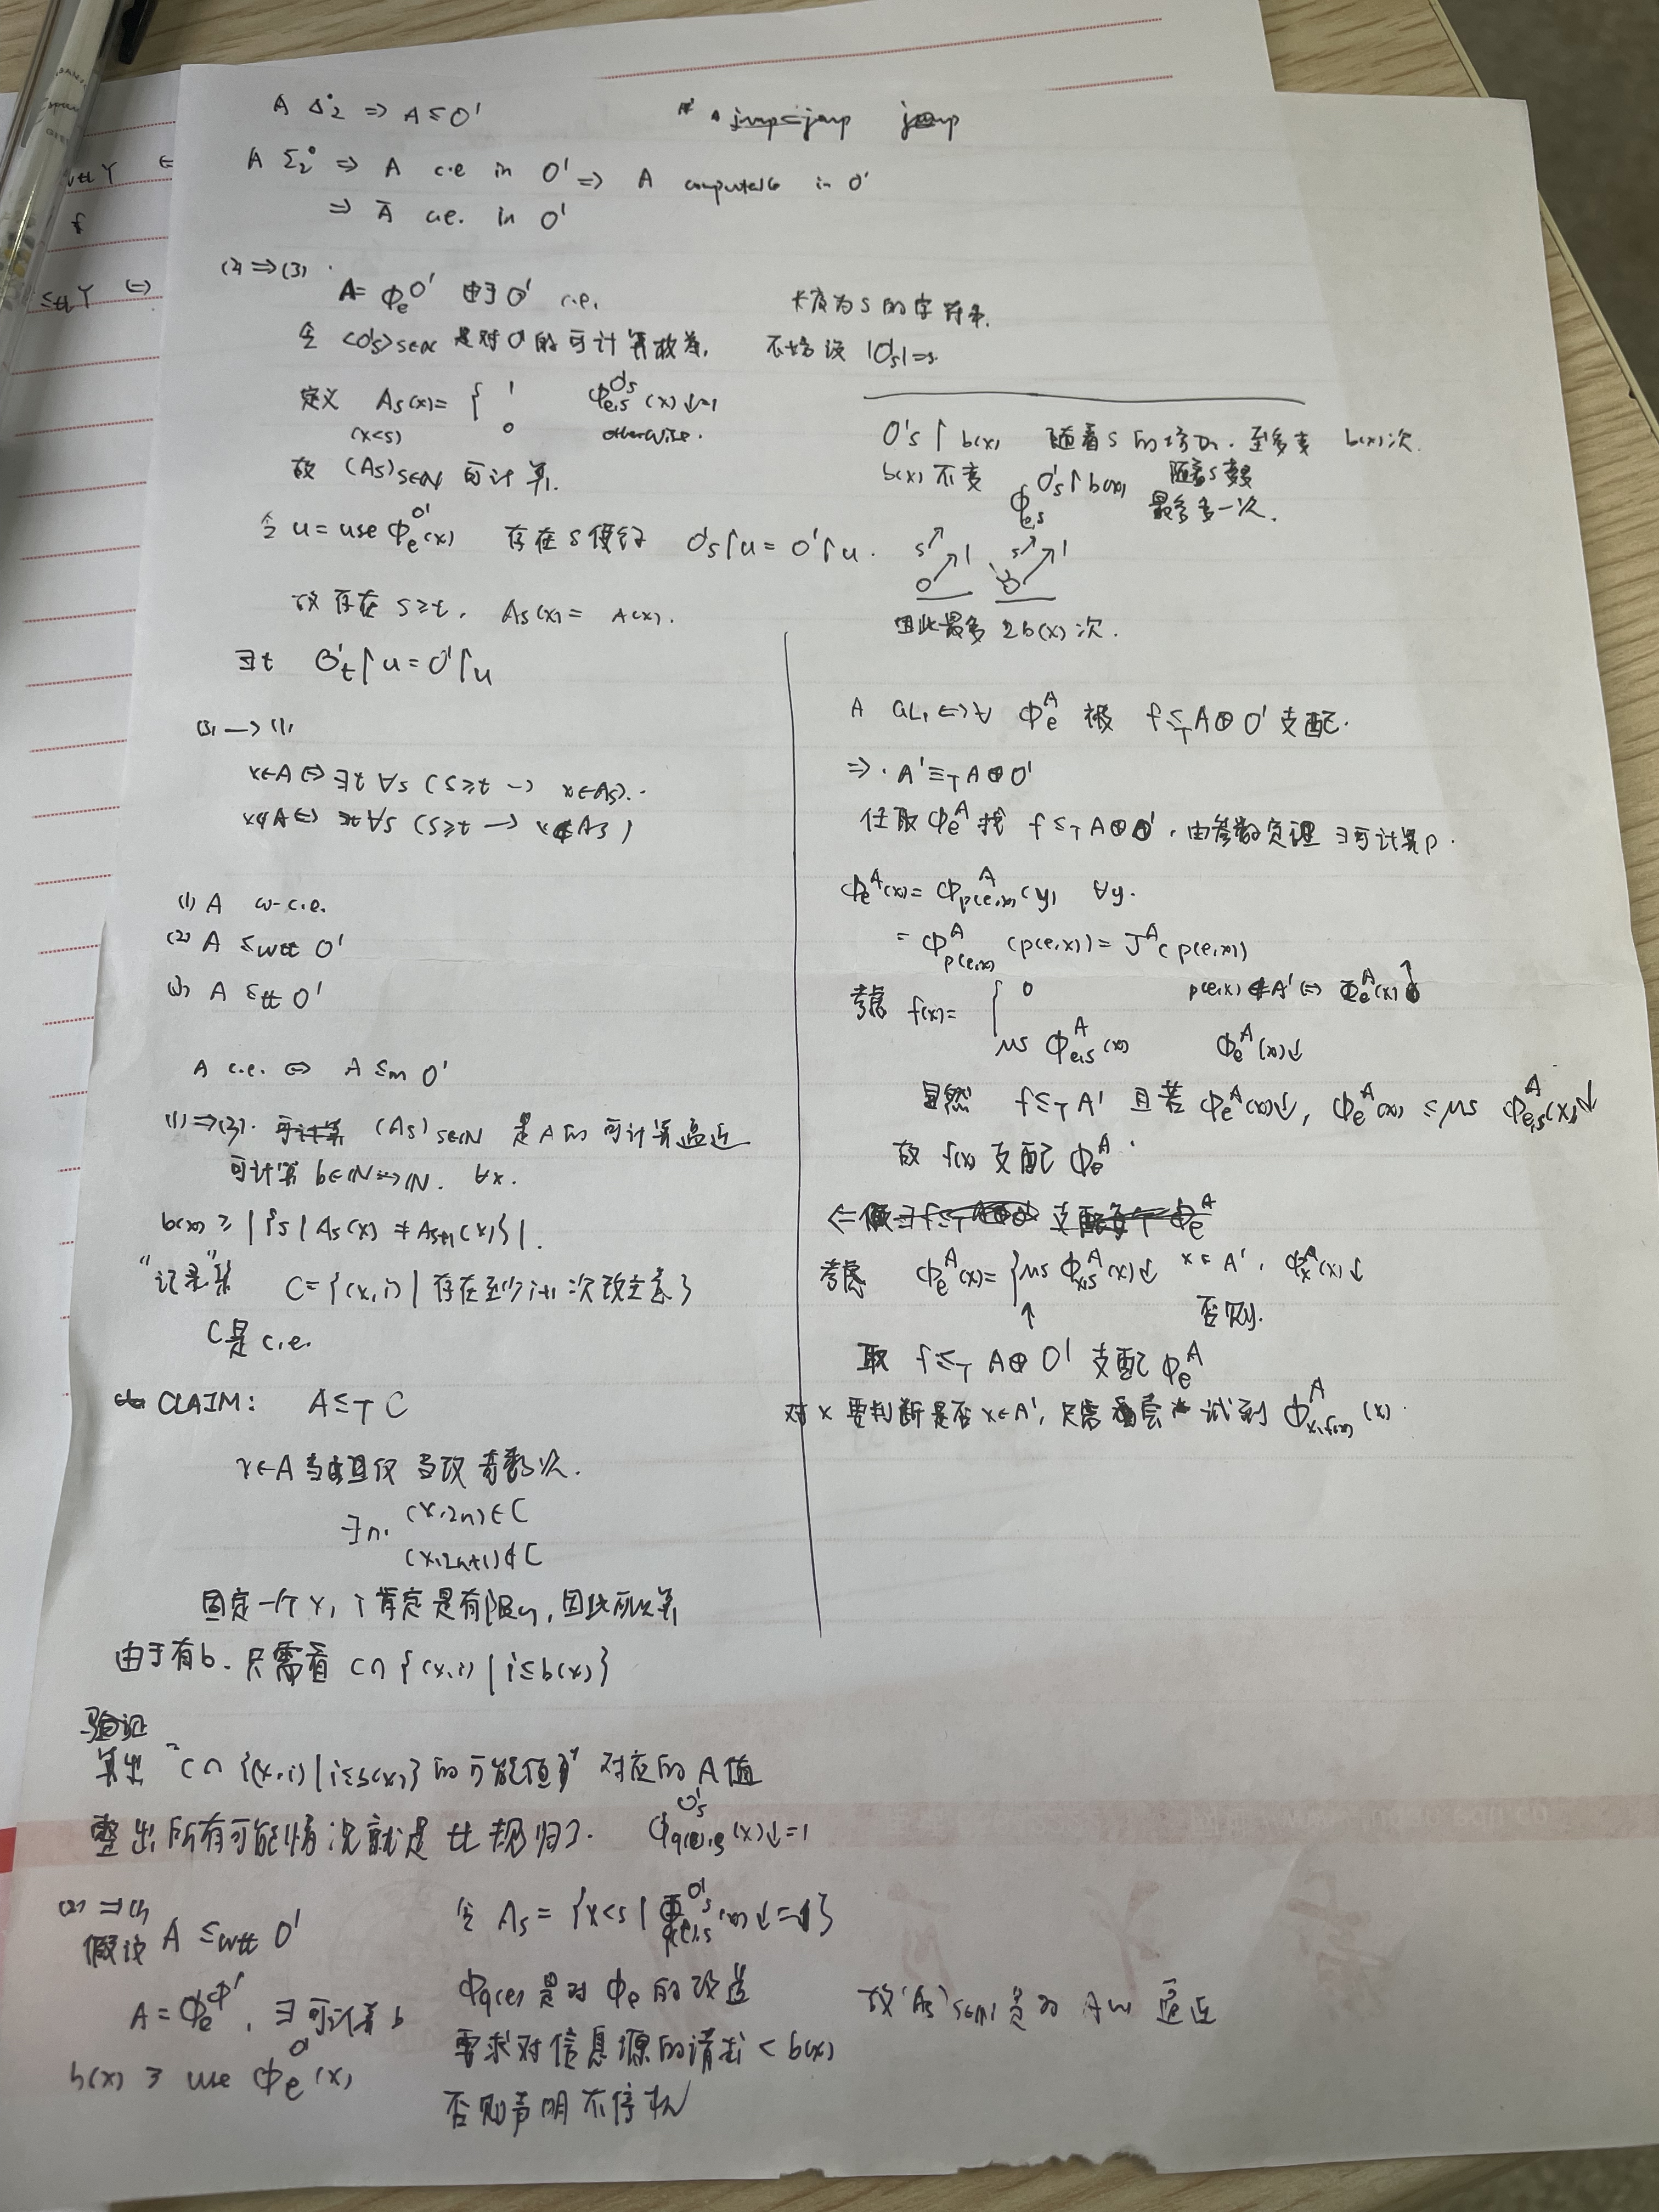
\includegraphics[width=.6\textwidth]{./1.png}
\label{}
\end{figure}
The TM \(\tilde{M}\) encodes \(k\) tapes of \(M\) on a single tape by using
locations \(1,k+1,2k+1,\dots\) to encode the first tape, locations \(2,k+2,2k+2,\dots\) to
encode the second tape etc. For every symbol \(a\) in \(M\)'s alphabet, \(\tilde{M}\) will
contain both the symbol \(a\) and the symbol \(\hat{a}\). In the encoding of each tape, exactly
one symbol will be of the ``\^{} type'', indicating that the corresponding head of \(M\) is
positioned in that location. \(\tilde{M}\) will not touch the first \(n+1\) locations of its
tape (where the input is located) but rather start by taking \(O(n^2)\) steps to copy the input
bit by bit into the rest of the tape, while encoding it in the above way.
\end{proof}

\begin{remark}[Oblivious Turing machines]
One can ensure that the proof of Proposition \ref{prop1.6} yields a TM \(\tilde{M}\) with the
following property: its head movements do not depend on the input but only depend on the input
length. That is, every input \(x\in\{0,1\}^*\) and \(i\in\N\), the location of each of \(M\)'s
at the \(i\)th step of execution on input \(x\) is only a function of \(\abs{x}\) and \(i\). A
machine with this property is called \textbf{oblivious}.
\end{remark}

\href{https://www.youtube.com/watch?v=LZmFYR2q4g4}{link}

\begin{exercise}
\label{ex1.5}
Define a TM \(M\) to be \textbf{oblivious} if its head movements do not depend on the input but only on
the input length. That is, \(M\) is oblivious if for every input \(x\in\{0,1\}^*\) and \(i\in\N\), the
location of each of \(M\)'s heads at the \(i\)th step of execution on input \(x\) is only a
function of \(\abs{x}\) and \(i\). Show that for every time-constructible \(T:\N\to\N\),
if \(L\in\DTIME(T(n))\), then there is an oblivious TM that decides \(L\) in time \(O(T(n)^2)\).
Furthermore, show that there is such a TM that uses only \textbf{two tapes}: one input tape and one
work/output tape
\end{exercise}

\begin{proof}
We can construct an oblivious TM M' such that L(M)=L(M') using a technique similar to that in
the proof of Claim 1.6.

Observe that (1) after n steps, M's tape heads will all be in the position range [-n, n], and
(2) since M runs in time O(T(n)), there exists some constant k such that for every input n, M
runs n fewer than k*T(n) steps.

First, add two additional work tapes T\textsubscript{1} and T\textsubscript{2}. The first thing M' does is count the length of
the input and write it to T\textsubscript{1}. Next, write k*T(n) to T\textsubscript{2}. Since T is time-constructible, and we
have the value of 'n' on T\textsubscript{1}, this takes time at most T(n).

Next, we simulate the execute of M in an oblivious way. We simulate each step i of M's execution as follows:
\begin{itemize}
\item Start every head t position -i. Move it right to position +i, finding the tape-head-location
marker along the way (See Claim 1.6). We note the tapes's movement, writes, and state
transition and then return to -(i+1) to begin the next step. If a tape's head is to move
right, do so on the right pass, otherwise remember and when we see the marker on the way back,
move it at that time. The write and state change can be made on the first pass.
\item Simultaneously, decrement the value on T\textsubscript{2}.
\end{itemize}

When T\textsubscript{2} is 0, halt.

The proof of language equality is essentially the same as in Claim 1.6, and obliviousness is
apparent. Waiting k*T(n) simulated steps to halt guarantees that all machines of this input
length would have halted by then.

Time anlaysis:
\begin{enumerate}
\item Writing T\textsubscript{1}, incrementing one-by-one, takes time n*log(n). (For each symbol in the input, we
may have to manipulate up to log(n) inputs of the length-so-far's binary representation to increment the value.)
\item Writing T\textsubscript{2} takes time T(n), by the definition of time-constructible
\item Each simulation step, the tapes move up to O(T(n)) steps. Keeping track of -i and i can be
done on another tape that simply counts in unary, with the head moving across it to count out
the correct distance.
\item Decrementing T\textsubscript{2} takes O(log(k*T(n))) = O(log(T(n))) steps
\item Multiplying c+d by the O(T(n)) ``simulated steps'' gets us O(T(n))*O(T(n) + log(T(n))) =
O(T(n)*T(n) + log(T(n))*T(n)), and since and log(T(n)) < T(n), this simulation runs in
O(T(n)**2)
\end{enumerate}

It remains to show that this simulation can be done in as few as 2 tapes. To do this, we interleave all tapes other than the input tape in the standard way.
\begin{itemize}
\item Writing T\textsubscript{1} is only a constant factor slower.
\item Similarly with writing T\textsubscript{2}, since these are performed sequentially with no other non-input tapes active.
\item Each simulation step is also only a constant-factor slower, since we can run over all the interleaved tapes at once, and the T\textsubscript{2} decrement is performed sequentially afterward.
\end{itemize}
\end{proof}


\subsubsection{The Class \texorpdfstring{\(P\)}{P}}
\label{sec:orgf712763}
A \textbf{complexity class} is a set of function that can be computed within given resource bounds.

We say that a machine \textbf{decides} a language \(L\subseteq\{0,1\}^*\) if it computes the
function \(f_L:\{0,1\}^*\to\{0,1\}\) where \(f_L(x)=1\Leftrightarrow x\in L\)

\begin{definition}[]
Let \(T:\N\to\N\) be some function. A language \(L\) is in \(\DTIME(T(n))\) iff there is a
Turing machine that runs in \(c\dot T(n)\) for some constant \(c>0\) and decides \(L\).
\end{definition}

The D in \(\DTIME\) refers to ``deterministic''.

\begin{definition}[]
\(\bP=\bigcup_{c\ge1}\DTIME(n^c)\)
\end{definition}

\section{Chap 2: NP and NP completeness}
\label{sec:orgaddc209}

\subsubsection{The Class \(\NP\)}
\label{sec:org9377e18}
\begin{definition}[]
A language \(L\subseteq\{0,1\}^*\) is in \(\NP\) if there exists  a polynomial \(p:\N\to\N\)
and a polynomial-time TM \(M\) (called the \textbf{verifier} for \(L\)) s.t. for
every \(x\in\{0,1\}^*\)
     \begin{equation*}
x\in L\Leftrightarrow \exists u\in\{0,1\}^{p(\abs{x})}\text{ s.t. }M(x,u)=1
     \end{equation*}
If \(x\in L\) and \(u\in\{0,1\}^{p(\abs{x})}\) satisfy \(M(x,u)=1\) then we call \(u\) a
\textbf{certificate} for \(x\)
\end{definition}

\begin{examplle}[\(\INDSET\in\NP\)]
By representing the possible invitees to a dinner party with the vertices of a graph having an
edge between any two people who don't get along. The dinner party computational problem becomes
the problem of finding a maximum sized \textbf{independent set} (set of vertices without any common
edges) in a given graph. The corresponding language is
     \begin{equation*}
\INDSET=\{\la G,k\ra:\exists S\subseteq V(G)\text{ s.t. }\abs{S}\ge k\text{ and }\forall u,v\in S, \ove{uv}\not\in E(G)\}
     \end{equation*}

Consider the following polynomial-time algorithm \(M\): Given a pair \(\la G,k\ra\) and a
string \(u\in\{0,1\}^*\), output 1 iff \(u\) encodes a list of \(k\) vertices of \(G\) s.t.
there is no edge between any two members of the list. Note that if \(n\) is the number of
vertices in \(G\), then a list of \(k\) vertices can be encoded using \(O(k\log n)\) bits,
where \(n\) is the number of vertices in \(G\). Thus \(u\) is a string of at
most \(O(n\log n)\) bits, which is polynomial in the size of the representation of \(G\).
\end{examplle}

\begin{proposition}[]
Let \(\EXP=\bigcup_{c>1}\DTIME(2^{n^c})\). Then \(\bP\subseteq\NP\subseteq\EXP\)
\end{proposition}

\begin{proof}
\(\bP\subseteq\NP\). Suppose \(L\in\bP\) is decided in polynomial-time by a TM \(N\).
Then we take \(N\) as the machine \(M\) and make \(p(x)\) the zero polynomial

\(\NP\subseteq\EXP\). We can decide \(L\) in time \(2^{O(p(n))}\)  by enumerating all
possible \(n\) and using \(M\) to check whether \(u\) is a valid certificate for the
input \(x\). Note that \(p(n)=O(n^c)\) for some \(c>1\), the number of choices for \(u\) is \(2^{O(n^c)}\).
\end{proof}

\(\NP\) stands for \textbf{nondeterministic polynomial time}.

NDTM has \textbf{two} transition function \(\delta_0\) and \(\delta_1\), and a special state denoted
by \(q_{\accept}\). When an NDTM \(M\) computes a function, we envision that at each
computational step \(M\) makes an arbitrary choice at to which of its two transition functions
to apply. For every input \(x\), we say that \(M(x)=1\) if there \textbf{exists} some sequence of this
choices that would make \(M\) reach \(q_{\accept}\) on input \(x\). We say that \(M\) runs
in \(T(n)\) time if for every input \(x\in\{0,1\}^*\) and every sequence of nondeterministic
choices, \(M\) reaches the halting state or \(q_{\accept}\) within \(T(\abs{x})\) steps

\begin{definition}[]
For every function \(f:\N\to\N\) and \(L\subseteq\{0,1\}^*\) we say that \(L\in\NTIME(T(n))\)
if there is a constant \(c>0\) and a \(c\dot T(n)\)-time NDTM \(M\) s.t. for
every \(x\in\{0,1\}^*\), \(x\in L\Leftrightarrow M(x)=1\)
\end{definition}

\begin{theorem}[]
\(\NP=\bigcup_{c\in\N}\NTIME(n^c)\)
\end{theorem}

\begin{proof}
The main idea is that the sequence of nondeterministic choices made by an accepting computation
of an NDTM can be viewedas a certificate that the input is in the language, and vice versa

Suppose \(p:\N\to\N\) is a polynomial and \(L\) is decidable by a NDTM \(N\) that runs in
time \(p(n)\). For every \(x\in L\), there is a sequence of nondeterministic choices that
makes \(N\) reach \(q_{\accept}\) on input \(x\). We can use this sequence as a certificate
for \(x\). This certificate has length \(p(\abs{x})\) and can be verified in polynomial time by
a deterministic machine.

Conversely, if \(L\in\NP\), then we describe a polynomial time NDTM \(N\) that decides \(L\).
On input \(x\), it uses the ability to make nondeterministic choices to write down a
string \(u\) of length \(p(\abs{x})\). (Having transition \(\delta_0\) correspond to writing a
0 and \(\delta_1\) ). Then it runs the deterministic verifier
\end{proof}

\subsubsection{Reducibility and NP-Completeness}
\label{sec:org5c65f89}
\begin{definition}[]
A language \(L\subseteq\{0,1\}^*\) is \textbf{polynomial-time Karp reducible to a
language} \(L'\subseteq\{0,1\}^*\) (sometimes shortened to just ``polynomial-time reducible''), denoted
by \(L\le_p L'\) if there is a polynomial-time
computable function \(f:\{0,1\}^*\to\{0,1\}^*\) s.t. for every \(x\in\{0,1\}^*\),
\(x\in L\) iff \(f(x)\in L'\)

We say that \(L'\) is \textbf{\(\NP\)-hard} if \(L\le_pL'\) for every \(L\in\NP\). We say that \(L'\)
is \textbf{\(\NP\)-complete} if \(L'\) is \(\NP\)-hard and \(L'\in\NP\)
\end{definition}

\begin{theorem}[]
\begin{enumerate}
\item (Transitivity) If \(L\le_pL'\) and \(L'\le_pL''\) then \(L\le_pL''\)
\item If language \(L\) is \(\NP\)-hard and \(L\in\bP\) then \(\bP=\NP\)
\item If language \(L\) is \(\NP\)-complete, then \(L\in\bP\) iff \(\bP=\NP\)
\end{enumerate}
\end{theorem}

\begin{theorem}[]
The following language is \(\NP\)-complete
    \begin{equation*}
\TMSAT=\{\la\alpha,x,1^n,1^t\ra:\exists u\in\{0,1\}^n\text{ s.t. }M_\alpha\text{ outputs }1
\text{ on input }\la x,u\ra\text{ within }t\text{ steps}\}
    \end{equation*}
\end{theorem}

\begin{proof}
There is a polynomial \(p\) and a verifier TM \(M\) s.t. \(x\in L\) iff there is a
string \(u\in\{0,1\}^{p(\abs{x})}\) satisfying \(M(x,u)=1\) and \(M\) runs in time \(q(n)\) for
some polynomial \(q\).

Map every string \(x\in\{0,1\}^*\) to the tuple \(\la\lcorner{M},x,1^{p(\abs{x})},1^{q(m)}\)
where \(m=\abs{x}+p(\abs{x})\) and \(\lcorner{M}\) denotes the representation of \(M\) as
string.
    \begin{align*}
&\la\lcorner{M},x,1^{p(\abs{x})},1^{q(m)}\ra\in\TMSAT\\
&\Leftrightarrow\exists u\in\{0,1\}^{p(\abs{x})}\text{ s.t. }M(x,u)\text{ outputs 1 within }q(m)\text{ steps}\\
&\Leftrightarrow x\in L
    \end{align*}
\end{proof}

\subsubsection{The Cook-Levin Theorem: Computation is Local}
\label{sec:orgb1e025d}
We denote by \(\SAT\) the language of all satisfiable CNF formulae and by \(\TSAT\) the
language of all satisfiable 3CNF formulae

\begin{theorem}[Cook-Levin Theorem]
\label{thm2.10}
\begin{enumerate}
\item \(\SAT\) is \(\NP\)-complete
\item \(\TSAT\) is \(\NP\)-complete
\end{enumerate}
\end{theorem}

\begin{lemma}[Universality of AND, OR, NOT]
\label{lemma2.13}
For every Boolean function \(f:\{0,1\}^l\to\{0,1\}\), there is an \(l\)-variable CNF formula \(\varphi\)
of size \(l2^l\) s.t. \(\varphi(u)=f(u)\) for every \(u\in\{0,1\}^l\), where the size of a CNF
formula is defined to be the number of \(\wedge/\vee\) symbols it contains
\end{lemma}

\begin{proof}
For every \(v\in\{0,1\}^l\), there exists a clause \(C_v(z_1,\dots,z_l)\) s.t. \(C_v(v)=0\)
and \(C_v(u)=1\) for every \(u\neq v\).

We let \(\varphi\) be the AND of all the clauses \(C_v\) for \(v\) s.t. \(f(v)=0\)
     \begin{equation*}
\varphi=\bigwedge_{v:f(v)=0}C_v(z_1,\dots,z_l)
     \end{equation*}
Note that \(\varphi\) has size at most \(l2^l\).
\end{proof}

\begin{lemma}[]
\(\SAT\) is \(\NP\)-hard
\end{lemma}

\begin{proof}
Let \(L\) be an \(\NP\) language. By definition, there is a polynomial time TM \(M\) s.t. for
every \(x\in\{0,1\}^*\), \(x\in L\Leftrightarrow M(x,u)=1\) for
some \(u\in\{0,1\}^{p(\abs{x})}\), where \(p:\N\to\N\) is some polynomial. We show \(L\) is
polynomial-time Karp reducible to \(\SAT\) by describing a polynomial-time
transformation \(x\to\varphi_x\) from strings to CNF formulae s.t. \(x\in L\) iff \(\varphi_x\)
is satisfiable. Equivalently
     \begin{equation*}
\varphi_x\in\SAT \quad\text{ iff }\quad\exists u\in\{0,1\}^{p(\abs{x})}
\text{ s.t. }M(x\circ u)=1
     \end{equation*}
where \(\circ\) denotes concatenation

Assume \(M\)
\begin{enumerate}
\item \(M\) only has two tapes - an input tape and a work/output tape
\item \(M\) is an oblivious TM in the sense that its head movement does not depend on the contents
of its tapes. That is, \(M\)'s computation takes the same time for all inputs of size \(n\),
and for every \(i\) the location of \(M\)'s head at the \(i\)th step depends only on \(i\)
and the length of the input
\end{enumerate}


We can make these assumptions without loss of generality because for every \(T(n)\)-time TM \(M\)
there exists a two-tape oblivious TM \(\tilde{M}\) computing the same function
in \(O(T(n)^2)\). Thus in particular, if \(L\in\NP\), then there exists a two-tape oblivious
polynomial-time TM \(M\) and a polynomial \(p\) s.t.
     \begin{equation}
     \label{eq:2.2}
x\in L \Leftrightarrow \exists u\in\{0,1\}^{p(\abs{x})}\text{ s.t. }M(x\circ u)=1
     \end{equation}

Note that because \(M\) is oblivious, we can run it on the trivial input \((x,0^{p(\abs{x})})\)
to determine the precise head position of \(M\) during its computation on every other input of
the same length.

Denote by \(Q\) the set of \(M\)'s possible states and by \(\Gamma\) its alphabet. The \textbf{snapshot}
of \(M\)'s execution on some input \(y\) at a particular step \(i\) is the triple
\(\la a,b,q\ra\in\Gamma\times\Gamma\times Q\) s.t. \(a,b\) are the symbols read by \(M\)'s
heads from the two tapes and \(q\) is the state \(M\) is in at the \(i\)th step. Clearly the
snapshot can be encoded as a binary string. Let \(c\) denote the length of this string, which
is some constant depending upon \(\abs{Q}\) and \(\abs{\Gamma}\)

\begin{center}
\includegraphics[width=.5\textwidth]{./5.png}
\end{center}

For every \(y\in\{0,1\}^*\), the snapshot of \(M\)'s execution on input \(y\) at the \(i\)th
step depends on its state in the \((i-1)\)st step and the contents of the current cells of its
input and work tapes.

Suppose somebody were to claim the existence of some \(u\) satisfying \(M(x\circ u)=1\) and as
evidence, present you with the sequence of snapshots that arise from \(M\)'s execution
on \(x\circ u\). How can you tell that the snapshots present a valid computation that was
actually performed by \(M\).

Clearly, it suffices to check that for each \(i\le T(n)\), the snapshot \(z_i\) is correct
given the snapshot for the previous \(i-1\) steps. However, since the TM can only read/modify
one bit at a time, to check the correctness of \(z_i\) it suffices to look at only \emph{two} of the
previous snapshots. Specifically, to check \(z_i\) we need to only look at the following:
\(z_{i-1}\), \(y_{\text{inputpos}(i)}\), \(z_{\text{prev}(i)}\).

\begin{center}
\includegraphics[width=.8\textwidth]{./2.png}
\end{center}

Here \(y\) is a shorthand
for \(x\circ u\). \(\text{inputpos}(i)\) denotes the location of \(M\)'s input tape head at
the \(i\)th step. \(\text{prev}(i)\) is the last step before \(i\) when \(M\)'s head was in the
same cell on its work tape that it is during step \(i\). The reason this small amount of
information suffices to check the correctness of \(z_i\) is that the contents of the current
cell have not been affected between step \(\text{prev}(i)\) and step \(i\).

Since \(M\) is a deterministic TM, for every triple of values
to \(z_{i-1},y_{\text{inputpos}(i)}\), \(z_{\text{prev}(i)}\), there is at most one value
of \(z_i\) that is correct. Thus there is some function \(F\) that maps \(\{0,1\}^{2c+1}\)
to \(\{0,1\}^c\) s.t. a correct \(z_i\) satisfies
     \begin{equation*}
z_i=F(z_{i-1},z_{\text{prev}(i)},y_{\text{inputpos}(i)})
     \end{equation*}

Because \(M\) is oblivious, the values \(\text{inputpos}(i)\) and \(\text{prev}(i)\) do not
depend on the particular input \(i\). These indices can be computed in polynomial-time by
simulating \(M\) on a trivial input.

By \eqref{eq:2.2} , \(x\in\{0,1\}^{n}\in L\) iff \(M(x\circ u)=1\) for
some \(u\in\{0,1\}^{p(n)}\). The previous discussion shows this latter condition occurs iff
there exists a string \(y\in\{0,1\}^{n+p(n)}\) and a sequence of strings
\(z_1,\dots,z_{T(n)}\in\{0,1\}^c\) (where \(T(n)\) is the number of steps \(M\) takes on inputs
of length \(n+p(n)\)) satisfying the following four conditions
\begin{enumerate}
\item The first \(n\) bits of \(y\) are equal to \(x\)
\item The string \(z_1\) encodes the initial snapshot of \(M\). That is, \(z_1\) encodes the
triple \(\la\rhd,\Box,q_{\start}\ra\).
\item For every \(i\in\{2,\dots,T(n)\}\), \(z_i=F(z_{i-1},z_{\text{prev}(i)},y_{\text{inputpos}(i)})\).
\item The last string \(z_{T(n)}\) encodes a snapshot where the machine halts and outputs 1
\end{enumerate}


The formula \(\varphi_x\) will take variables \(y\in\{0,1\}^{n+p(n)}\)
and \(z\in\{0,1\}^{cT(n)}\) and will verify that \(y,z\) satisfy the AND of these four
conditions. Thus \(x\in L\Leftrightarrow\varphi_x\in\SAT\).

Condition 1 can be expressed as a CNF formula of size \(4n\) . Conditions 2 and 4 each depend
on \(c\) variables and hence by Proposition \ref{lemma2.13} can be expressed by CNF formulae of
size \(c2^c\). Condition 3, which is an AND of \(T(n)\) conditions each  depending on at most \(3c+1\)
variables, can be expressedas a CNF formula of size at most \(T(n)(3c+1)2^{3c+1}\). Hence the AND of all
these conditions can be expressed as a CNF formula of size d(n + T(n)) where d is some constant
depending only on \(M\). Moreover, this CNF formula can be computed in time polynomial in the running
time of \(M\).
\end{proof}

\begin{lemma}[]
\(\SAT\le_p\TSAT\)
\end{lemma}

\begin{proof}
Suppose \(\varphi\) is a 4CNF. Let \(C\) be a clause of \(\varphi\), say \(C=u_1\vee\baru_2\vee\baru_3\vee u_4\).
We add a new variable \(z\) to the \(\varphi\) and replace \(C\) with the pair
\(C_1=u_1\vee\baru_2\vee z\) and \(C_2=\baru_3\vee u_4\vee\barz\). If \(C\) is true, then there
is an assignment to \(z\) that satisfies both \(C_1\) and \(C_2\). If \(C\) is false, then no
matter what value we assign to \(z\) either \(C_1\) or \(C_2\) will be false.

For every clause \(C\) of size \(k>3\), we change it into an equivalent pair of clauses \(C_1\)
of size \(k-1\) and \(C_2\) of size 3.
\end{proof}


\subsubsection{The Web of Reductions}
\label{sec:org570a3fa}
\begin{center}
\includegraphics[width=.8\textwidth]{./3.png}
\end{center}

A \textbf{Hamilton path} in a directed graph is a path that visits all vertices exactly once. Let
\(\dHAMPATH\) denote the set of all directed graphs that contain such a path
\begin{theorem}[]
\(\dHAMPATH\) is \(\NP\)-complete
\end{theorem}

\begin{proof}
\begin{center}
\includegraphics[width=.8\textwidth]{./4.png}
\end{center}

The graph \(G\) has
\begin{enumerate}
\item \(m\) vertices for each of \(\varphi\)'s clause \(c_1,\dots,c_m\)
\item a special starting vertex \(v_{\start}\) and ending vertex \(v_{\tend}\)
\item \(n\) ``chains'' of \(4m\) vertices corresponding to the \(n\) variables of \(\varphi\) . A chain is a
set of vertices \(v_1,\dots,v_{4m}\) s.t. for every \(i\in[1,4m-1]\), \(v_i\)
and \(v_{i+1}\) are connected by two edges in both directions
\end{enumerate}


If \(C\) contains the literal \(u_j\), then we take two neighboring
vertices \(v_i\), \(v_{i+1}\) in the \(j\)th chain and put an edge from \(v_i\) to \(C\) and
from \(C\) to \(v_{i+1}\). If \(C\) contains the literal \(\baru_j\) then we construct these
edges in the opposite direction. When adding these edges, we never ``reuse'' a
link \(v_i, v_{i+1}\) in a particular chain and always keep an unused link between every two
used links.


\(G\in\dHAMPATH\Rightarrow\varphi\in\SAT\). Suppose that \(G\) has an Hamiltonian path \(P\).
We first note that the path \(P\) must start in \(v_{\start}\) and end at \(v_{\tend}\).
Furthermore, we claim that \(P\) needs to traverse all the chains in order and, within each
each chain, traverse it either in left-to-right order or right-to-left order.
\end{proof}
\end{document}
